\documentclass{beamer}
 
\usepackage [T2A,T1] {fontenc}
\usepackage[utf8]{inputenc}
\usepackage[english,russian]{babel}
\usepackage{listings}
\usepackage{xcolor}
\usepackage{graphbox}
\usepackage{tikz}

\setbeamertemplate{navigation symbols}{}

\usetikzlibrary{arrows,shapes,decorations.markings,positioning}

\tikzstyle{entity} = [rectangle, minimum width=0.5cm, minimum height=3cm, text width=2cm, text centered, draw=black, fill=blue!20]
\tikzstyle{file} = [rectangle, minimum height=1.5cm, text width=1cm, text centered, draw=black, fill=orange!30]
\tikzstyle{tool} = [rectangle, rounded corners, minimum width=0.5cm, text width=1cm, text centered, draw=black, fill=green!20]

\tikzstyle{vecArrow} = [thick, decoration={markings,mark=at position
   1 with {\arrow[semithick]{open triangle 60}}},
   double distance=1.4pt, shorten >= 5.5pt,
   preaction = {decorate},
   postaction = {draw,line width=1.4pt, white,shorten >= 4.5pt}]
\tikzstyle{innerWhite} = [semithick, white,line width=1.4pt, shorten >= 4.5pt]

\definecolor{base3}{RGB}{253,246,227}
\definecolor{base2}{RGB}{238,232,213}
\definecolor{base1}{RGB}{147,161,161}
\definecolor{base00}{RGB}{101	,123,131}

\lstset{
  backgroundcolor=\color{base3},
  basicstyle=\ttfamily\tiny,
  commentstyle=\color{base1},
  frame=single,
  keywordstyle=\color{blue},
  stringstyle=\color{magenta}
}

\lstnewenvironment{cmdline}
  {\lstset{basicstyle=\ttfamily,keywordstyle=\color{blue},
           language={bash}}}
  {}
 
\title[C++]
{Программирование на языке C++}
 
\subtitle{Вводный курс}
 
\author[А.~Б.~Морозов]
{
  \texorpdfstring{Александр Морозов\newline\href{mailto:gelu.speculum@gmail.com}{gelu.speculum@gmail.com}}
  {Александр Морозов}
}
  
\date[ITMO 2019]
{ИТМО, весенний семестр 2019}
 
\logo{%
  \makebox[0.95\paperwidth]{%
    
\includegraphics[align=c,width=1.5cm,keepaspectratio]{itmo_logo.png}
    \hfill
    
\includegraphics[align=c,width=0.9cm,keepaspectratio]{itiviti_logo.png}
  }
}

\AtBeginSection[]
{
  \begin{frame}
    \frametitle{Содержание}
    \tableofcontents[currentsection]
  \end{frame}
}

\begin{document}
 
\frame{\titlepage}

%-------------------------------------------------
\section{Вступление}

\begin{frame}{О чём этот курс?}
\begin{itemize}
  \item Основные элементы языка C++ \vspace{3em}
  \item Некоторые инструменты для разработки программ на C++ \vspace{3em}
  \item Базовые навыки программирования \vspace{3em}
\end{itemize}
\end{frame}

\begin{frame}{Почему C++?}
\begin{itemize}
  \item Язык сочетает черты низкоуровневого и высокоуровневого \vspace{1em}
  \item Позволяет как использовать сложные абстракции, так и прибегать к низкоуровневым оптимизациям и ручному управлению ресурсами \vspace{1em}
  \item Zero overhead abstractions \vspace{1em}
  \item Значительно более высокоуровневый, чем C, но в то же время может быть настолько же эффективным \vspace{1em}
  \item Один из самых распространенных прикладных языков \vspace{1em}
\end{itemize}
\end{frame}

\begin{frame}{Формат курса}
  \begin{itemize}
    \item Лекции \vspace{1em}
    \item Небольшие примеры-иллюстрации к лекциям \vspace{1em}
    \item Практические задания (необходимо выполнить 3 любых в течении семестра) \vspace{1em}
    \item Доклады по желанию \vspace{1em}
    \item Сдача задач через code review на github.com \vspace{1em}
  \end{itemize}
\end{frame}

\begin{frame}{Некоторая литература}
\begin{itemize}
  \item Bjarne Stroustrup: Programming: Principles and Practice Using C++, 2014\\Программирование Принципы и практика использования С++
  \item Bjarne Stroustrup: The C++ Programming Language (Special edition), 2000\\Язык программирования C++ Специальное издание
  \item Bjarne Stroustrup: The Design and Evolution of C++, 1994\\Дизайн и эволюция C++
  \item Stanley Lippman: C++ Primer (5th Edition), 2012\\Язык программирования C++. Базовый курс
  \item Herb Sutter: Exceptional C++, 1999; More Exceptional C++, 2001\\Решение сложных задач на С++
\end{itemize}
\end{frame}

%-------------------------------------------------
\section{История}

\begin{frame}{Первые языки программирования}
Машинные коды\\
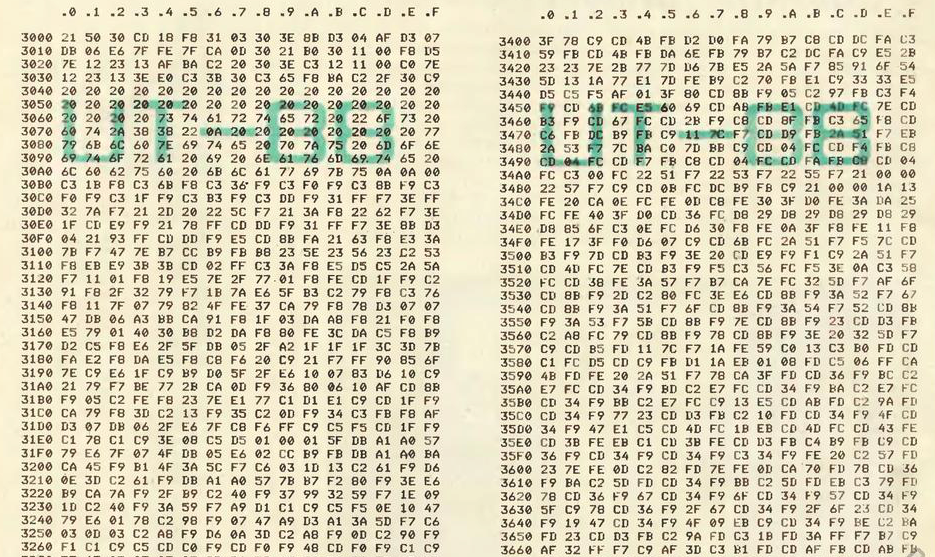
\includegraphics[keepaspectratio]{history/ut88.png}\\
{\tiny Из <<ЮТ для умелых рук, 1990/2>>}
\end{frame}

\begin{frame}[fragile]{Первые языки программирования}
Ассемблер\\
\lstinputlisting[language={[x86masm]Assembler}]{history/foo.asm}
\end{frame}

\begin{frame}{Первые языки программирования}
\begin{itemize}
  \item FORTRAN: язык математических вычислений, 1954
  \item LISP: язык списков, первый <<гомоиконный>> язык, 1958
  \item COBOL: бизнес-ориентированный язык, 1959
  \item ALGOL: процедурный язык, 1960
  \item BASIC: учебный язык, 1963
  \item PL/I: язык обработки данных, 1964
  \item Simula: объектно-ориентированный язык, 1965
  \item C: эффективный процедурный язык, 1972
  \item Prolog: язык логического программирования, 1972
  \item ML: функциональный язык с автоматическим выводом типов и формально доказуемой типобезопасностью, 1973
\end{itemize}
\end{frame}

\begin{frame}{Классификация языков программирования}
\begin{itemize}
  \item Компилируемые / интерпретируемые
  \item Императивные / декларативные
  \item Поддержка различных парадигм: ООП, функциональные, логические
  \item Статическая типизация / динамическая типизация
  \item Сильная типизация / слабая типизация
  \item Энергичные / ленивые
\end{itemize}
\end{frame}

\begin{frame}{Появление C++: цели создателя}
Бьярне Страуструп занимался моделированием распределенных аспектов операционных систем и ему нужен был язык:
\begin{itemize}
  \item ООП
  \item пользовательские абстракции
  \item сильная типизация
  \item эффективность
  \item отсутствие <<необоснованной стоимости>> возможностей
  \item простота реализации (использование уже существующих инструментов)
  \item отсутствие излишних ограничений на стиль программирования
\end{itemize}
\end{frame}

\begin{frame}{Краткая история C++}
1979 - C with classes (расширение языка C классами, наследованием, более сильной типизацией, встраиваемыми функциями).

1983 - C++ (перегрузка функций и операторов, виртуальные функции, ссылки, типобезопасное управление памятью).

1985 - The C++ Programming Language (первое описание языка).

1989 - C++ 2.0 (множественное наследование, абстрактные классы, статические члены классов).

1990 - The Annotated C++ Reference Manual (шаблоны, исключения, пространства имен).

1992 - STL (обобщенная реализация различных структур данных и типовых алгоритмов).

1998 - C++98, первый ISO стандарт языка.
\end{frame}

\begin{frame}{Краткая история C++, продолжение}
1999 - Boost.

2003 - C++03, второй ISO стандарт, незначительные изменения.

2011 - С++11, новый стандарт, большие изменения и модернизация.

2013 - 4-е издание The C++ Programming Language.

2014 - C++14, дальнейшее развитие нового стандарта.

2017 - C++17, текущий стандарт языка.
\end{frame}

\begin{frame}{Место C++ в современном мире}
\begin{itemize}
  \item Графические редакторы и среды 3D моделирования (Photoshop, Maya)
  \item Компьютерные игры (CryEngine, Frostbite, Gamebryo, id Tech 4-, Source, Unreal Engine)
  \item CAD (Autodesk, Catia)
  \item Браузеры и Javascript движки (Chrome, Firefox, V8, SpiderMonkey)
  \item Базы данных (MongoDB, частично MS SQL, Oracle, SAP DB)
  \item Системы информационного поиска, интернет поисковики (Google, Яндекс)
  \item Финтех (Bloomberg, Morgan Stanley, Itiviti)
\end{itemize}
\end{frame}

%-------------------------------------------------
\section{Абстрактная вычислительная машина}

\begin{frame}[t]{Абстрактная машина vs Настоящее железо}
\scriptsize
\begin{columns}[t]
\begin{column}{0.5\textwidth}
  \begin{itemize}
    \item Архитектура фон Неймана: общая память, АЛУ, УУ
    \item Последовательное исполнение
    \item Линейная непрерывная память
    \item Числа определяются в человеческих понятиях (целые, рациональные и т.п.)
  \end{itemize}
\end{column}
\begin{column}{0.5\textwidth}
  \begin{itemize}
    \item Особенности конкретной архитектуры, например, big-ending vs little-endian; битность процессора
    \item Целые и дробные числа представляются по-разному
    \item Много уровней памяти: регистры, кеш нескольких уровней, RAM
    \item Реальный и защищенный режим
    \item Виртуальная память
    \item Прерывания, системные вызовы, переключение контекста
    \item Параллелизм: внутри ядра процессора, между несколькими ядрами, между процессорами; разные гарантии синхронизации на разных архитектурах
    \item Инструкции различной сложности: RISC, CISC, векторные инструкции, сопроцессоры (“математический”, GPU)
  \end{itemize}
\end{column}
\end{columns}
\normalsize
\end{frame}

\begin{frame}{Абстракции до C++11}
\begin{itemize}
  \item Последовательное исполнение в рамках observable behaviour
  \item Параллелизм отсутствует
  \item Целые числа подчиняются определенным правилам, без подробностей реализации
  \item Беззнаковые целые числа немного ближе к аппаратным подробностям
  \item Дробные числа имеют определенную точность и диапазон
  \item Исключения заданы лишь высокоуровневым поведением, без особенностей реализации
  \item Есть понятие упаковки сложных объектов в памяти, padding, требования к размещению в памяти заданы обтекаемо, в стандарте нет возможностей на это влиять
\end{itemize}
\end{frame}

\begin{frame}{Что изменилось в C++11}
\begin{itemize}
  \item Появилась модель памяти, учитывающая параллельное исполнение \vspace{3em}
  \item Управление многопоточностью добавлено в стандартную библиотеку \vspace{3em}
  \item Конструкции для высокоуровневого управления параллелизмом \vspace{3em}
\end{itemize}
\end{frame}

%-------------------------------------------------
\section{Пример программы на C++}

\begin{frame}[fragile]{Пример программы на C++}
\lstinputlisting[language={[11]C++}]{examples/hello_world.cpp}
\end{frame}

%-------------------------------------------------
\section{Инструментарий}

\begin{frame}{Трансляция}
\begin{figure}
\begin{tikzpicture}[node distance=4cm, auto,>=latex', thick]

\node (source) [entity] {Текст программы};
\node (executable) [entity, right of=source] {?};

\draw[vecArrow] (source) -- node[anchor=south] {?} (executable);
\draw[innerWhite] (source) -- (executable);

\end{tikzpicture}
\end{figure}
\end{frame}

\begin{frame}{3 этапа трансляции C++}
\begin{figure}
\begin{tikzpicture}[node distance=2.5cm, auto,>=latex', thick]

\node (src) [file] {\tiny .cpp};
\node (cpp) [tool, below of=src] {\hspace{0pt}\tiny Препроцессор};
\node (tmp) [file, below of=cpp] {\tiny tmp};
\node (c++) [tool, right of=tmp] {\hspace{0pt}\tiny Компилятор};
\node (asm) [file, above of=c++] {\tiny .s};
\node (as) [tool, above of=asm] {\hspace{0pt}\tiny Ассемблер};
\node (obj) [file, right of=as] {\tiny .o};
\node (linker) [tool, below of=obj] {\hspace{0pt}\tiny Компоновщик};
\node (exe) [file, below of=linker] {\hspace{0pt}\tiny executable};
\node (lib) [file, right of=linker] {\hspace{0pt}\tiny Библиотеки};

\draw[vecArrow] (src) -- (cpp);
\draw[innerWhite] (src) -- (cpp);

\draw[vecArrow] (cpp) -- (tmp);
\draw[innerWhite] (cpp) -- (tmp);

\draw[vecArrow] (tmp) -- (c++);
\draw[innerWhite] (tmp) -- (c++);

\draw[vecArrow] (c++) -- (asm);
\draw[innerWhite] (c++) -- (asm);

\draw[vecArrow] (asm) -- (as);
\draw[innerWhite] (asm) -- (as);

\draw[vecArrow] (as) -- (obj);
\draw[innerWhite] (as) -- (obj);

\draw[vecArrow] (obj) -- (linker);
\draw[innerWhite] (obj) -- (linker);

\draw[vecArrow] (linker) -- (exe);
\draw[innerWhite] (linker) -- (exe);

\draw[vecArrow] (lib) -- (linker);
\draw[innerWhite] (lib) -- (linker);

\end{tikzpicture}
\end{figure}
\end{frame}

\begin{frame}[fragile]{Трансляция C++ на примере gcc}
Трансляция программы из одного файла:
\begin{cmdline}
g++ -std=c++17 -o prog prog.cpp
\end{cmdline}
Результат препроцессора:
\begin{cmdline}
g++ -std=c++17 -E prog.cpp
\end{cmdline}
Ассемблерный код:
\begin{cmdline}
g++ -std=c++17 -S prog.cpp
\end{cmdline}
Объектный файл:
\begin{cmdline}
g++ -std=c++17 -c prog.cpp
\end{cmdline}
\end{frame}

\begin{frame}{Гарантии языка и undefined behaviour}
\begin{itemize}
  \item Некоторые вещи язык гарантирует - вне зависимости от платформы, компилятора и иных внешних факторов. Например, \lstinline[basicstyle=\ttfamily\small]{sizeof(int) <= sizeof(long)}.
  \item \emph{Observable behaviour}: компилятор может менять программу, если её внешнее поведение не меняется.
  \item \emph{Implementation defined behaviour}: поведение программы может различаться в зависимости от реализации компилятора (но это должно быть задокументировано).
  \item \emph{Unspecified behaviour}: поведение зависит от реализации, но это не требуется документировать; каждый возможный вариант поведение должен быть корректным.
  \item \emph{Undefined behaviour}: стандарт не накладывает никаких ограничений на поведение в этом случае.
\end{itemize}
\end{frame}

\begin{frame}{Объектные файлы}
Объектные файлы обычно состоят из различных секций. Например: заголовок, секция кода, секция данных, отладочная информация.

Сущности ссылаются по именам, адреса в памяти не назначены.

Mangling: имена сущностей из текста программы не всегда могут быть перенесены в имена в объектном файле. Для C обычно соответствие точное (хотя некоторые реализации добавляют к имени дополнительную информацию). В C++ структура имен более сложная и они приводятся к уникальным строковым именам по определенному алгоритму (зависит от реализации).\\
Например, имя \lstinline[basicstyle=\ttfamily\small]{Space::Outer::Inner::code} может быть преобразовано в \lstinline[basicstyle=\ttfamily\small]{_ZN5Space5Outer5Inner4codeE}.
\end{frame}

\begin{frame}{Online компиляторы}
\begin{itemize}
  \item Coliru  \href{https://coliru.stacked-crooked.com/}{https://coliru.stacked-crooked.com/} \vspace{3em}
  \item Wandbox  \href{https://wandbox.org/}{https://wandbox.org/} \vspace{3em}
  \item Godbolt  \href{https://godbolt.org/}{https://godbolt.org/} \vspace{3em}
\end{itemize}
\end{frame}

\end{document}
